\chapter{后端优化及闭环检测}
\label{chap:4}
在初始化完成后,采用基于滑动窗口的紧耦合单目VIO进行高精度和鲁棒性的状态估计。后端非线性优化是实现视觉/惯性紧耦合的关键步骤,闭环检测能够实现系统的重定位,提高系统的鲁棒性。本章将对后端非线性优化算法、闭环检测算法以及闭环优化算法进行详细分析与研究。
\section{后端非线性优化}
\subsection{状态向量和目标函数}
滑动窗口中的所有状态向量定义为:
\begin{equation}
\label{eqn:4.1}{\tiny }
\begin{split}
\mathcal{X}&=[\mathbf{x}_0,\mathbf{x}_1,\cdots\mathbf{x}_n,\mathbf{x}_c^b,\lambda_0,\lambda_1,\cdots\lambda_m] \\
\mathbf{x}_k&=[\mathbf{p}_{b_k}^w,\mathbf{v}_{b_k}^w,\mathbf{q}_{b_k}^w,\mathbf{b}_a,\mathbf{b}_g],k\in[0,n] \\
\mathbf{x}_c^b&=[\mathbf{p}_c^b,\mathbf{q}_c^b],
\end{split}
\end{equation}
其中 $\mathbf{x}_k $ 是第 $k$ 帧图像关联的IMU状态,它包含了IMU在世界坐标系中的位置、速度和方向,以及在IMU坐标系中的加速度计bias和陀螺仪bias, $n$ 是关键帧的总数,$m$ 是滑动窗口中的路标点总数,$\lambda_l$ 是第一次观测到的第 $l$ 个路标的逆深度(深度的倒数)。$\mathbf{x}_c^b $ 是外参。

定义目标函数为所有先验项和测量残差的马氏范数(Mahalanobis Norm)之和,从而得到最大后验概率估计:
\begin{equation}
\label{eqn:4.2}
\begin{split}
\underset{\mathcal{X}}{\text{min}}
\left\{
\left\| 
\mathbf{r}_p-\mathbf{H}_p\mathcal{X} 
\right\|^2+
\sum_{k\in\mathcal{B}}
\left\| 
\mathbf{r}_\mathcal{B}(\hat{\mathbf{z}}_{b_{k+1}}^{b_k},\mathcal{X}) 
\right\|
_{\mathbf{p}_{b_{k+1}}^{b_k}}^2+ \right. 
\left.\sum_{(l,j)\in\mathcal{C}}\rho(
\left\| 
\mathbf{r}_\mathcal{C}(\hat{\mathbf{z}}_l^{c_j},\mathcal{X}) 
\right\|
_{\mathbf{p}_l^{c_j}}^2) 
\right\}
\end{split}
\end{equation}
其中$\mathbf{r}_\mathcal{B}(\hat{\mathbf{z}}_{b_{k+1}}^{b_k},\mathcal{X})  $ 和 $\mathbf{r}_\mathcal{C}(\hat{\mathbf{z}}_l^{c_j},\mathcal{X})  $ 分别是IMU和视觉测量的残差。$\mathcal{B} $ 是所有IMU测量的集合,$\mathcal{C} $ 是在当前滑动窗口中至少观察到两次的一组特征。$\left\{ \mathbf{r}_p,\mathbf{H}_p\right\} $ 是来自边缘化的先验信息。$\rho (\cdot) $ 为:
\begin{equation}
\label{eqn:4.3}
\rho(s)=
\left\{\begin{array}{lc}
s & s\leq 1,\\
2\sqrt{s}-1 & s\textgreater 1.
\end{array}\right. 
\end{equation}
将 $\left\| \mathbf{r}_\mathcal{C} \right\|^2 $ 代入式(\ref{eqn:4.3})得:
\begin{equation}
\label{eqn:4.4}
\frac{1}{2}\rho( \left\| \mathbf{r}_\mathcal{C} \right\| )=\left\{\begin{array}{lc}
\frac{1}{2} \left\| \mathbf{r}_\mathcal{C} \right\|^2 & |\mathbf{r}_\mathcal{C}| \leq 1,\\
\left\| \mathbf{r}_\mathcal{C}\right\| - \frac{1}{2} & |\mathbf{r}_\mathcal{C}| \textgreater 1.
\end{array}\right. 
\end{equation}
令 $e=\left\| \mathbf{r}_\mathcal{C} \right\|  $ ,则式(\ref{eqn:4.4})可变形为,
\begin{equation}
\label{eqn:4.5}
\begin{split}
H(e)=\left \{
\begin{array}{ll}
\frac12 e^2, & e \leq 1,\\
|e| - \frac12, & e \textgreater 1.
\end{array}
\right.
\end{split}
\end{equation}
 $H(e) $是胡贝尔(Huber)核函数\upcite{huber1992robust}。Huber核函数是鲁棒核函数得一种,使用核函数是为了避免异常的误差值对整个目标函数的影响。因为当误差很大时,二范数(或马氏范数)增长太快,导致这种异常的误差项掩盖掉其他正确得误差项。图4.1展示了Huber核函数与二次函数的图像对比,可见当误差较大时,Huber核函数的增长速度要低于二次函数。
 \begin{figure}[h]\setlength{\belowcaptionskip}{-12pt}
 	\centering
 	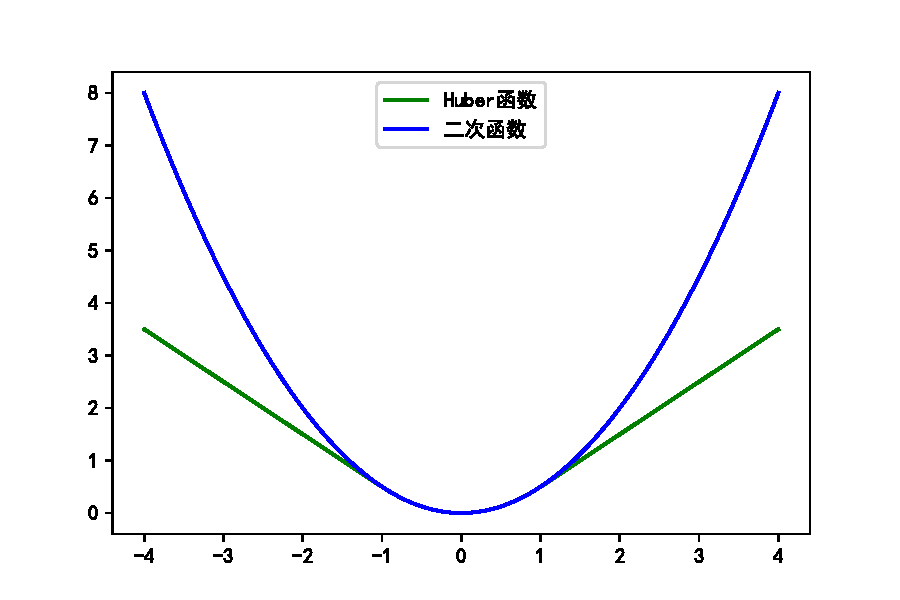
\includegraphics[width=0.45\textwidth]{figures/chapter4/fig4_1}
 	\caption{Huber函数与二次函数图像}\label{fig4_1}
 \end{figure}


需要注意的是,使用马氏范数而不是二范低于因为马氏范数消除了不同残差项的尺度不一致性(单位/量纲不一致性),或者说马氏范数对残差项的概率模型进行了归一化,从而使得不同的残差项可以直接相加。

要计算目标函数的最小值,使用迭代优化的思想,每次给优化变量一个增量,使得目标函数最小。对于IMU残差项,
\begin{equation}
\label{eqn:4.6}
\begin{aligned}
& \min _{\delta X}\left\| \mathbf{r}_\mathcal{B}(\hat{\mathbf{z}}_{b_{k+1}}^{b_k}, \mathcal{X} + \Delta \mathcal{X} )  \right\|_{P_{b_{k+1}}^{b_k}}^{2} \\
&=
\min _{\delta X} 
\left\| 
\mathbf{r}_\mathcal{B}(\hat{\mathbf{z}}_{b_{k+1}}^{b_k},\mathcal{X}) 
+ \mathbf{J}_{b_{k+1}}^{b_k} \Delta \mathcal{X}  \right\| _{P_{b_{k+1}}^{b_k}}^{2}
\end{aligned}
\end{equation}
其中$\mathbf{J}_{b_{k+1}}^{b_k}  $ 是IMU残差项 $\mathbf{r}_{\mathcal{B}} $ 关于状态向量 $\mathcal{X} $ 的雅可比矩阵。上式可以展开成 $\mathbf{H}\Delta \mathbf{x}=\mathbf{b} $ 的形式:
\[
(\mathbf{J} _{b_{k+1}}^{b_{k}})^{T} (\mathbf{P}_{b_{k+1}}^{b_{k}})^{-1} \mathbf{J}_{b_{k+1}}^{b_{k}} \Delta \mathcal{X}
=- (\mathbf{J}_{b_{k+1}}^{b_{k}})^{T} (\mathbf{P}_{b_{k+1}}^{b_{k}})^{-1} \mathbf{r}_{B}
\]
其中$\mathbf{P}_{b_{k+1}}^{b_k} $ 是IMU预积分中噪声项的协方差矩阵。

同理,可以写出视觉残差项的增量方程。整体目标函数的增量方程为:
\begin{equation}
\label{eqn:4.7}
\begin{aligned}
& \left( \mathbf{H}_{p}+\sum (\mathbf{J}_{b_{k+1}}^{b_{k}})^{T} (\mathbf{P}_{b_{k+1}}^{b_{k}})^{-1} \mathbf{J}_{b_{k+1}}^{b_{k}}+\sum {\mathbf{J}_{l}^{C_{j}}}^{T}  (\mathbf{P}_{l}^{C_j})^{-1}  \mathbf{J}_{l}^{C_{j}}\right) \Delta \mathcal{X} \\
& = \mathbf{b}_{p}+\sum \mathbf{J}_{b_{k+1}}^{b_{k}} (\mathbf{P}_{b_{k+1}}^{b_{k}})^{-1} \mathbf{r}_{B}+\sum {\mathbf{J}_{l}^{C_{j}} }^T  (\mathbf{P}_{l}^{C_j})^{-1}  \mathbf{r}_{C}
\end{aligned}
\end{equation}
其中$\mathbf{P}_{l}^{C_{j}} $ 是视觉噪声的协方差。暂时不考虑先验信息,用 $(\mathbf{H}_p, \mathbf{b}_p) $ 表示。称 ${\mathbf{P}_{b_{k+1}}^{b_{k}}}^{-1} $ 为信息矩阵,其大小可以代表IMU测量数据的可靠程度,越大代表越可靠,越小代表越不可靠。可以观察到,IMU噪声越大,信息矩阵就越小,此时IMU观测量就越不可靠,可以直观的理解为目标函数“更加相信”视觉的观测量。

将增量方程(\ref{eqn:4.7})简化为:
\begin{equation}
\label{eqn:4.8}
\setlength{\abovedisplayskip}{6pt}
\setlength{\belowdisplayskip}{6pt}
\left( \bm{\Lambda}_{p}+\bm{\Lambda}_{\mathcal{B}}+\bm{\Lambda}_{\mathcal{C}} \right) \Delta \mathcal{X}=\mathbf{b}_{p}+\mathbf{b}_{\mathcal{B}}+\mathbf{b}_{\mathcal{C}}
\end{equation}
其中$\bm{\Lambda}_{p}, \bm{\Lambda}_{\mathcal{B}}, \bm{\Lambda}_{\mathcal{C}} $ 分别为先验残差项,IMU残差项和视觉残差项的海森(Hessian)矩阵。
\subsection{IMU约束}
考虑滑动窗口中连续两帧图像( $b_{k} $和 $b_{k+1} $)内的IMU测量,根据式(3.41)中定义的IMU测量模型,预积分残差可以定义为:
\begin{equation}
\label{eqn:4.9}
\begin{split}
\mathbf{r}_\mathcal{B}(\hat{\mathbf{z}}_{b_{k+1}}^{b_k},\mathcal{X})=\begin{bmatrix} \delta\bm{\alpha}_{b_{k+1}}^{b_k} \\ \delta\bm{\beta}_{b_{k+1}}^{b_k} \\ \delta\bm{\theta}_{b_{k+1}}^{b_k} \\ \delta\mathbf{b}_a \\ \delta\mathbf{b}_g  \end{bmatrix}  
=\begin{bmatrix}
\mathbf{R}_w^{b_k}(\mathbf{p}_{b_{k+1}}^w-\mathbf{p}_{b_k}^w+\frac{1}{2}\mathbf{g}^w\Delta t_k^2-\mathbf{v}_{b_k}^w\Delta t_k)-\hat{\bm{\alpha}}_{b_{k+1}}^{b_k} \\
\mathbf{R}_w^{b_k}(\mathbf{v}_{b_{k+1}}^w+\mathbf{g}^w\Delta t_k^2-\mathbf{v}_{b_k}^w)-\hat{\bm{\beta}}_{b_{k+1}}^{b_k} \\
2\left[ {\mathbf{q}_{b_k}^w}^{-1}\otimes\mathbf{q}_{b_{k+1}}^w\otimes(\hat{\bm{\gamma}}_{b_{k+1}}^{b_k})^{-1} \right]_{xyz} \\ \mathbf{b}_{ab_{k+1}}-\mathbf{b}_{ab_k} \\
\mathbf{b}_{wb_{k+1}}-\mathbf{b}_{wb_k}
\end{bmatrix}
\end{split}
\end{equation}
其中$[\cdot]_{x y z}$ 表示四元数的向量。$\delta \boldsymbol{\theta}_{b_{k+1}}^{b_{k}}$ 是四元数对应的三维误差状态。$\left[\hat{\boldsymbol{\alpha}}_{b_{k+1}}^{b_{k}}, \hat{\boldsymbol{\beta}}_{b_{k+1}}^{b_{k}}, \hat{\gamma}_{b_{k+1}}^{b_{k}}\right]^{T}$ 是在两个连续图像帧之间的间隔时间内带有噪声的预积分IMU测量项。$\delta \mathbf{b}_a, \delta \mathbf{b}_g $ 是加速度计bias和陀螺仪bias的误差。

IMU残差项的优化变量为:
\[
\setlength{\abovedisplayskip}{6pt}
\setlength{\belowdisplayskip}{6pt}
\left[ \mathbf{ p}_{b_{k}}^{w}, 
\mathbf{ q}_{b_{k}}^{w}\right],
\left[\mathbf{ v}_{b_{k}}^{w}, 
\mathbf{ b}_{a_{k}}, \mathbf{ b}_{\omega_{k}}\right], 
\left[\mathbf{ p}_{b_{k+1}}^{w}, \mathbf{q}_{b_{k+1}}^{w}\right],
\left[\mathbf{ v}_{b_{k+1}}^{w}, \mathbf{ b}_{a_{k+1}}, \mathbf{b}_{\omega_{k+1}}\right]
\]

在进行迭代优化时需要知道残差项对优化变量的一阶导数,也就是雅可比矩阵,以及协方差矩阵。仍旧采用扰动模型求导,扰动为:
\[
\setlength{\abovedisplayskip}{6pt}
\setlength{\belowdisplayskip}{6pt}
\left[\delta \mathbf{p}_{b_{k}}^{w},   \delta \bm{\theta}_{b_{k}}^{w}\right], 
\left[\delta \mathbf{v}_{b_{k}}^{w},   \delta \mathbf{b}_{a_{k}}, \delta \mathbf{b}_{\omega_{k}}\right], 
\left[\delta \mathbf{p}_{b_{k+1}}^{w}, \delta \bm{\theta}_{b_{k+1}}^{w}\right],
\left[\delta \mathbf{v}_{b_{k+1}}^{w}, \delta \mathbf{b}_{a_{k+1}}, \delta \mathbf{b}_{\omega_{k+1}}\right]
\]

这里直接给出通过扰动模型求导后的雅可比矩阵:
\begin{equation}
\label{eqn:4.10}
\begin{aligned}
\mathbf{J}[0]^{15 \times 7} &= \left[\frac{\partial \mathbf{r}_{\mathcal{B}}}{\partial \mathbf{p}_{b_{k}}^{w}}, \frac{\partial \mathbf{r}_{\mathcal{B}}}{\partial \mathbf{q}_{b_{k}}^{w}}\right] \\
&= \left[\begin{array}{cc}
-\mathbf{R}_{w}^{b_{k}} & \left[ \mathbf{R}_{w}^{b_{k}}\left(\mathbf{p}_{b_{k+1}}^{w} - \mathbf{p}_{b_{k}}^{w} - \mathbf{v}_{b_{k}}^{w} \Delta t_{k}+\frac{1}{2} \mathbf{g}^{w} \Delta t_{k}^{2}\right) \right]_\times \\ 
\bm{0}                       & -{\left[ (\mathbf{q}_{b_{k+1}}^{w})^{-1} \otimes \mathbf{q}_{b_{k}}^{w}\right]}_L {\left[\bm{\gamma}_{b_{k+1}}^{b_{k}}\right]}_R \\
\bm{0}                       & \left[ \mathbf{R}_{w}^{b_{k}}\left(\mathbf{v}_{b_{k+1}}^{w} - \mathbf{v}_{b_{k}}^{w} + \mathbf{g}^{w} \Delta t_{k}\right) \right]_\times \\
\bm{0}                       &\bm{0}\\
\bm{0}                      & \bm{0}
\end{array}\right]
\end{aligned}
\end{equation}
\begin{equation}
\label{eqn:4.11}
\begin{aligned}
\mathbf{J}[1]^{15 \times 9} &= \left[\frac{\partial \mathbf{r}_{\mathcal{B}}}{\partial \mathbf{v}_{b_{k}}^{w}}, \frac{\partial \mathbf{r}_{\mathcal{B}}}{\partial \mathbf{b}_{k}}, \frac{\partial \mathbf{r}_{\mathcal{B}}}{\partial \mathbf{b}_{w_{k}}}\right] \\
&= \left[ \begin{array}{ccc}
{-\mathbf{R}_{w}^{b_{k}} \Delta t} & {-\mathbf{J}_{b_{a}}^{\alpha}} & {-\mathbf{J}_{b_{\omega}}^{\alpha}} \\ 
{\bm{0}} & {\bm{0}} & {\left[{\mathbf{q}_{b_{k+1}}^{w}}^{-1} \otimes \mathbf{q}_{b_{k}}^{w} \otimes \bm{\gamma}_{b_{k+1}}^{b_{k}}\right]_L \mathbf{J}_{b_{\omega}}^{\gamma}} \\ 
{-\mathbf{R}_{w}^{b_{k}}} & {-\mathbf{J}_{b_{a}}^{\beta}} & {-\mathbf{J}_{b_{\omega}}^{\beta}} \\ 
{\bm{0}} & {-\mathbf{I}} & {\bm{0}} \\ {\bm{0}} & {\bm{0}} & {\mathbf{-I}}\end{array}\right]
\end{aligned}
\end{equation}
\begin{equation}
\label{eqn:4.12}
\begin{aligned}
\mathbf{J}[2]^{15 \times 7} = \left[\frac{\partial \mathbf{r}_{\mathcal{B}}}{\partial \mathbf{p}_{b_{k+1}}^{w}}, \frac{\partial \mathbf{r}_{\mathcal{B}}}{\partial \mathbf{q}_{b_{k+1}}^{w}}\right] 
= \left[ \begin{array}{cc}
\mathbf{R}_{w}^{b_k} & {\bm{0}} \\ 
{\bm{0}} & \left[{\bm{\gamma}_{b_{k+1}}^{b_{k}}}^{-1} \otimes \mathbf{q}_{b_{k}}^{w-1} \otimes \mathbf{q}_{b_{k+1}}^{w}\right]_L \\ 
{\bm{0}} & {\bm{0}}  \\ 
{\bm{0}} & {\bm{0}} 
\end{array}\right]
\end{aligned}
\end{equation}
\begin{equation}
\label{eqn:4.13}
\mathbf{J}[3]^{15 \times 9}=\left[\frac{\partial \mathbf{r}_{\mathcal{B}}}{\partial \mathbf{v}_{b_{k+1}}^{w}}, \frac{\partial \mathbf{r}_{\mathcal{B}}}{\partial \mathbf{b}_{a_{k+1}}}, \frac{\partial \mathbf{r}_{\mathcal{B}}}{\partial \mathbf{b}_{w_{k+1}}}\right]
=\left[ \begin{array}{ccc}{\bm{0}} & {\bm{0}} & {\bm{0}} \\ {\bm{0}} & {\bm{0}} & {\bm{0}} \\ {\mathbf{R}_{w}^{b_{k}}} & {\bm{0}} & {\bm{0}} \\ {\bm{0}} & {\mathbf{I}} & {\bm{0}} \\ {\bm{0}} & {\bm{0}} & {\mathbf{I}}\end{array}\right]
\end{equation}

协方差矩阵是\ref{chap:3.2.3}小节中研究的预积分中的IMU增量误差的协方差矩阵,即公式(\ref{eqn:3.56})。
\subsection{视觉约束}
考虑第  $l$ 个特征,其对应的3D空间点为 $\mathbf{P}_l^{w} $ ,该特征在第 $i$  幅图像中被第一次观测到,观测到的像素坐标为 $ \mathbf{P}_{uv_{i}} =[u_l^{c_i},u_l^{c_j}]^{T} $ 。
\begin{equation}
\label{eqn:4.14}
\setlength{\abovedisplayskip}{6pt}
\setlength{\belowdisplayskip}{6pt}
\mathbf{P}_{uv_{i}}  =\lambda_{l} \pi_{c}\left( \mathbf{T}_{b \leftarrow c}^{-1} \mathbf{T}_{w \leftarrow b_{i}}^{-1} \mathbf{P}^w_{l}\right)
\end{equation}
其中$\pi_{c} $ 将世界坐标点映射为像素坐标点,$\mathbf{T}_{b \leftarrow c}^{-1} $ 将坐标从IMU系变换到相机系,$\mathbf{T}_{w \leftarrow b_{i}}^{-1} $ 将世界坐标系下的坐标变换到IMU坐标系下。$\lambda_l $ 是第 $l$ 个特征在第 $i$ 幅图像下的逆深度。由式(\ref{eqn:4.14})可得:
\begin{equation}
\label{eqn:4.15}
\begin{aligned}
\mathbf{P}^w_{l} &= \mathbf{T}_{w\leftarrow b_{i}} \mathbf{T}_{b\leftarrow c} \frac{1}{\lambda_{l}} \pi_{c}^{-1}\left( \mathbf{P}_{uv_{i}} \right) \\
&= \mathbf{R}_{b_{i}}^{w}\left(\mathbf{R}_{c}^{b} \frac{1}{\lambda_{l}} \pi_{c}^{-1}
\left(\left[ \begin{array}
{c}{u_{l}^{c_{i}}} \\ {v_{l}^{c_{i}}}
\end{array}\right]\right)
+ \mathbf{p}_{c}^{b}\right)+\mathbf{p}_{b_{i}}^{w}
\end{aligned}
\end{equation}
 $\mathbf{P}_l^{w} $ 在第 $j$ 副图像对应的相机坐标系下的坐标为,
\begin{equation}
\label{eqn:4.16}
\setlength{\abovedisplayskip}{6pt}
\setlength{\belowdisplayskip}{6pt}
\mathcal{ P}_{l}^{c_{j}}=\mathbf{T}_{b \leftarrow c}^{-1} \mathbf{T}_{w \leftarrow b_{j}}^{-1} \mathbf{P}_{l}^{w}
\end{equation}
进而得到,
\begin{equation}
\label{eqn:4.17}
\begin{aligned}
\mathbf{ P}_{l}^{w} &= \mathbf{T}_{w \leftarrow b_{j}} \mathbf{T}_{b \leftarrow c} \mathcal{P}_{l}^{c_{j}} \\
&= \mathbf{R}_{b_{j}}^{w}\left(\mathbf{R}_{c}^{b} \mathcal{P}_{l}^{c_{j}}+\mathbf{p}_{c}^{b}\right)+\mathbf{p}_{b_{j}}^{w}
\end{aligned}
\end{equation}
联立式(\ref{eqn:4.15})和(\ref{eqn:4.17})可得:
\begin{equation}
\label{eqn:4.18}
\mathcal{P}_l^{c_j}=\mathbf{R}_b^c(\mathbf{R}_w^{b_j}(\mathbf{R}_{b_i}^w(\mathbf{R}_c^b\frac{1}{\lambda_l}{\pi_c}^{-1}(\begin{bmatrix}  u_l^{c_j} \\ v_l^{c_j}
\end{bmatrix})+\mathbf{p}_c^b)+\mathbf{p}_{b_i}^w-\mathbf{p}_{b_j}^w)-\mathbf{p}_c^b)
\end{equation}

此时,可以定义该特征在第 $j$ 幅图像中的观测点和重投影点之间的残差定义为:
\begin{equation}
\label{eqn:4.19}
\mathbf{r}_\mathcal{C}(\hat{\mathbf{z}}_l^{c_j},\mathcal{X})= 
\hat{\bar{\mathcal{P}}}_l^{c_j}-\frac{ \mathcal{P}_l^{c_j} }{\left\|\mathcal{P}_l^{c_j}\right\|}
\end{equation}
其中$\mathcal{P}_l^{c_j} $ 为 $\mathbf{P}_l^{w} $ 在第 $j$ 副图像上对应的归一化平面坐标,
\begin{equation}
\label{eqn:4.20}
\hat{\bar{\mathcal{P}}}_l^{c_j}={\pi_c}^{-1}
(\begin{bmatrix}  \hat{u}_l^{c_j} \\ \hat{v}_l^{c_j}
\end{bmatrix})
\end{equation}
视觉残差项的优化变量为:
\[
\setlength{\abovedisplayskip}{6pt}
\setlength{\belowdisplayskip}{6pt}
\left[ \mathbf{p}_{b_{i}}^{w}, \mathbf{q}_{b_{i}}^{w}\right], 
\left[ \mathbf{p}_{b_{j}}^{w}, \mathbf{q}_{b_{j}}^{w}\right], 
\left[ \mathbf{p}_{c}^{b}, \mathbf{q}_{c}^{b}\right], 
\lambda_{l}
\]

同样需要计算残差项关于这些优化变量的一阶导数,得到其雅可比矩阵。这里直接给出各优化变量的雅可比矩阵:
\begin{equation}
\label{eqn:4.21}
\left\{
\begin{aligned}
\mathbf{ J}[0]^{3 \times 7} &= \left[\frac{\partial \mathbf{r}_{\mathcal{C}}}{\partial \mathbf{p}_{b_{i}}^{w}}, \frac{\partial \mathbf{r}_{\mathcal{C}}}{\partial \mathbf{q}_{b_{i}}^{w}}\right]
=\left[\mathbf{R}_{b}^{c} \mathbf{R}_{w}^{b_{j}}-\mathbf{R}_{b}^{c} \mathbf{R}_{w}^{b_{j}} \mathbf{R}_{b_{i}}^{w}\left[\mathbf{R}_{c}^{b} \frac{1}{\lambda_{l}} \hat{\bar{\mathcal{P}}}_{l}^{c_{i}}+\mathbf{p}_{c}^{b}\right]_\times\right] \\
\mathbf{J}[1]^{3 \times 7}&=\left[\frac{\partial \mathbf{r}_{\mathcal{C}}}{\partial \mathbf{p}_{b_{j}}^{w}}, \frac{\partial \mathbf{r}_{\mathcal{C}}}{\partial \mathbf{q}_{b_{j}}^{w}}\right] \\
&=\left[-\mathbf{R}_{b}^{c} \mathbf{R}_{w}^{b_{j}} \mathbf{R}_{b}^{c}\left[\mathbf{R}_{w}^{b_{j}}\left[\mathbf{R}_{b_{i}}^{w}\left(\mathbf{R}_{c}^{b} \frac{\hat{\bar{P}}_{l}^{c_{i}}}{\lambda_{l}}+\mathbf{p}_{c}^{b}\right)+\mathbf{p}_{b_{i}}^{w}-\mathbf{p}_{b_{j}}^{w}\right]\right]_\times\right] \\
\mathbf{J}[2]^{3 \times 7} &= \left[\frac{\partial \mathbf{r}_{\mathcal{C}}}{\partial \mathbf{p}_{\mathcal{C}}^{b}}, \frac{\partial \mathbf{r}_{\mathcal{C}}}{\partial \mathbf{q}_{c}^{b}}\right] \\
&= \left[ \begin{array}
{c}{\mathbf{R}_{b}^{c}\left(\mathbf{R}_{w}^{b_{j}} \mathbf{R}_{b_{i}}^{w}-\mathbf{I}_{3 \times 3}\right)} \\ 
\begin{aligned}
&{-\mathbf{R}_{b}^{c} \mathbf{R}_{w}^{b_{j}} \mathbf{R}_{b_{i}}^{w} \mathbf{R}_{c}^{b} \left[\frac{\hat{\bar{\mathcal{P}}}_{l}^{c_{i}}}{\lambda_{l}}\right]_\times
	+\left[\mathbf{R}_{b}^{c} \mathbf{R}_{w}^{b_{j}} \mathbf{R}_{b_{i}}^{w} \mathbf{R}_{c}^{b} \frac{\hat{\bar{\mathcal{P}}}_{l}^{c_{i}}}{\lambda_{l}}\right]_\times} \\
	&{+\left[\mathbf{R}_{b}^{c}\left[\mathbf{R}_{w}^{b_{j}}\left(\mathbf{R}_{b_{i}}^{w} \mathbf{p}_{c}^{b}+\mathbf{p}_{b_{i}}^{w}-\mathbf{p}_{b_{j}}^{w}\right)-\mathbf{p}_{c}^{b}\right]\right]_\times}
\end{aligned} \\
\end{array}\right]^{T} \\
\mathbf{J}[3]^{3 \times 1} &=\frac{\partial \mathbf{r}_{\mathcal{C}}}{\partial \lambda_{l}}=-\mathbf{R}_{b}^{c} \mathbf{R}_{w}^{b_{j}} \mathbf{R}_{b_{i}}^{w} \mathbf{R}_{c}^{b} \frac{\hat{\bar{P}}_{l}^{c_{i}}}{\lambda_{l}^{2}}
\end{aligned}
\right.
\end{equation}
\subsection{边缘化}
前面在研究残差项的时候,忽略了先验残差项,这个先验残差项就是通过边缘化(Marginalization)\upcite{Paz2008Divide}来的。整个后端是基于滑动窗口来进行非线性优化的,滑动窗口内的图像帧数量是固定的(在实际工程中取10帧),这样会带来一个问题:窗口在向前滑动的过程中,总会有新的图像帧和路标点进来,而窗口中最旧的图像帧和路标点会滑出窗口。要对滑窗内的所有图像位姿及其路标点进行优化,那么不能直接将最旧的图像帧及其观测到的路标点直接删除,因为这样会丢失观测信息,降维约束项。那么怎么才能在不减少约束项的情况下丢掉最旧的图像帧及其路标点呢?边缘化就是用来解决此问题的。

1. 舒尔补消元

采用高斯牛顿或者LM方法进行非线性优化时,每次迭代都需要求解增量方程 $\mathbf{H}\delta \mathbf{x}=\mathbf{b} $ ,将 $\mathbf{H}\delta \mathbf{x}=\mathbf{b} $ 写为:
\begin{equation}
\label{eqn:4.22}
\left[ \begin{array}{cc}
{\bm{\Lambda}_{a}} & {\bm{\Lambda}_{b}} \\ 
{\bm{\Lambda}_{b}^{T}} & {\bm{\Lambda}_{c}}
\end{array}\right] 
\left[ \begin{array}{c}
{\delta \mathbf{x}_{1}} \\ {\delta \mathbf{x}_{2}}
\end{array}\right]
=\left[ \begin{array}
{l}{\mathbf{b}_{1}} \\ {\mathbf{b}_{2}}
\end{array}\right]
\end{equation}
其中$\delta \mathbf{x}_1 $ 是想要边缘化掉的优化变量,$\delta \mathbf{x}_2 $ 是与 $\delta \mathbf{x}_1 $ 有约束关系的想要保留的优化变量。定义舒尔项\upcite{sibley2010sliding}:
\begin{equation}
\label{eqn:4.23}
\left[ \begin{array}{cc}
{\mathbf{I}} & {0} \\ 
{-\bm{\Lambda}_{b}^{T} \bm{\Lambda}_{a}^{-1}} & {\mathbf{I}}\end{array}\right]
\end{equation}
将等式(\ref{eqn:4.22})两边同时乘以式(\ref{eqn:4.23}),
\begin{equation}
\label{eqn:4.24}
\begin{aligned}
\left[ \begin{array}{cc}
{ \mathbf{I}} & {0} \\ 
{-\bm{\Lambda}_{b}^{T} \bm{\Lambda}_{a}^{-1}} & {\mathbf{I}}
\end{array}\right] 
\left[ \begin{array}{cc}
{\bm{\Lambda}_{a}} & {\bm{\Lambda}_{b}} \\ 
{\bm{\Lambda}_{b}^{T}} & {\bm{\Lambda}_{c}}
\end{array}\right] 
\left[ \begin{array}{c}
{\delta \mathbf{x}_{1}} \\ {\delta \mathbf{x}_{2}}
\end{array}\right]
&=
\left[ \begin{array}{cc}
{\mathbf{I}} & {0} \\ 
{-\bm{\Lambda}_{b}^{T} \bm{\Lambda}_{a}^{-1}} & {\mathbf{I}}
\end{array}\right] 
\left[ \begin{array}
{l}{\mathbf{b}_{1}} \\ {\mathbf{b}_{2}}
\end{array}\right] \\
\Longrightarrow
\left[ \begin{array}{cc}
{\bm{\Lambda}_{a}} & {\bm{\Lambda}_{b}} \\ 
{0} & {\bm{\Lambda}_{c}-\bm{\Lambda}_{b}^{T} \bm{\Lambda}_{a}^{-1} \bm{\Lambda}_{b}}
\end{array}\right] 
\left[ \begin{array}{l}
{\delta \mathbf{x}_{1}} \\ {\delta \mathbf{x}_{2}}
\end{array}\right]
&=
\left[ \begin{array}{c}
{\mathbf{b}_{1}} \\ {\mathbf{b}_{2}-\bm{\Lambda}_{\mathbf{b}}^{T} \bm{\Lambda}_{a}^{-1} \mathbf{b}_{1}}
\end{array}\right]
\end{aligned}
\end{equation}
通过式(\ref{eqn:4.24}),可以忽略 $\delta \mathbf{x}_1$ 单独求解 $\delta \mathbf{x}_2$,
\begin{equation}
\label{eqn:4.25}
\begin{aligned}
\left( \bm{\Lambda}_{c}-\bm{\Lambda}_{b}^{T} \bm{\Lambda}_{a}^{-1} \bm{\Lambda}_{b}\right) \delta \mathbf{x}_{2} &= 
b_{2}- \bm{\Lambda}_{b}^{T} \bm{\Lambda}_{a}^{-1} \mathbf{b}_{1} \\
\Longrightarrow  \quad \quad
\mathbf{H}^{*} \delta \mathbf{x}_{2}^{*}&= \mathbf{b}^{*}
\end{aligned}
\end{equation}
式(\ref{eqn:4.25})中,$\mathbf{b}^{*} $ 是 $\bm{\Lambda}_{b}^{T} \bm{\Lambda}_{a}^{-1} \mathbf{b}_{1} $有关的函数,所以,通过舒尔补,在保留了变量 $\delta \mathbf{x}_1 $ 的约束信息的情况下消掉了$\delta \mathbf{x}_1 $ 。因此可以说式(4.25)保留了变量 的先验信息。此时可以构建先验残差项:
\begin{equation}
\label{eqn:4.26}
\setlength{\abovedisplayskip}{6pt}
\setlength{\belowdisplayskip}{6pt}
\mathbf{r}_p-\mathbf{H}_p\mathcal{X} \Longleftrightarrow 
\hat{\mathbf{b}}^{*} - \mathbf{H}^{*} \delta \mathbf{x}_{2}^{*}
\end{equation}

2. 边缘化过程

假设相机在四个不同的地方拍摄了四张图像,相机的位姿分别为 $ \mathbf{x}_{p_1},  \mathbf{x}_{p_2},  \mathbf{x}_{p_3},  \mathbf{x}_{p_4} $ ,四张图像总共观测到了六个路标点 $ \mathbf{x}_{m_1},  \mathbf{x}_{m_2}, \mathbf{x}_{m_3}, \mathbf{x}_{m_4}, \mathbf{x}_{m_5}, \mathbf{x}_{m_6}$ ,他们之间的关系如图\ref{fig4_2}所示。
\begin{figure}[h]\setlength{\belowcaptionskip}{-12pt}
	\centering
	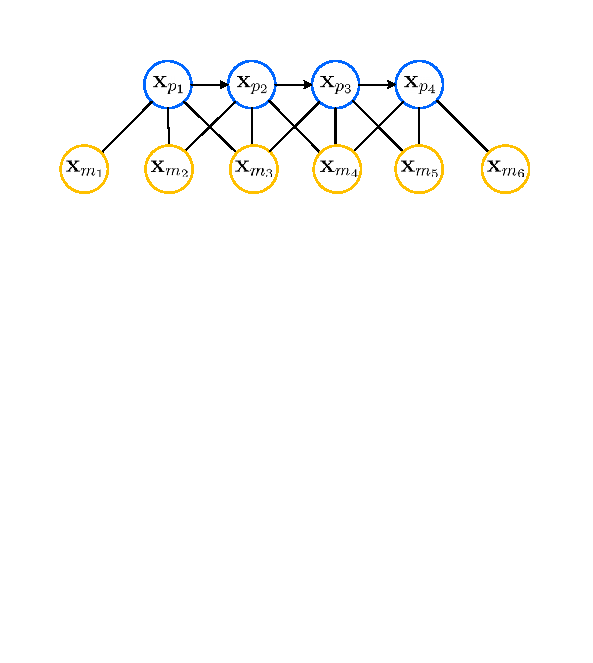
\includegraphics[width=0.15\textwidth, angle=-90]{figures/chapter4/fig4_2}
	\caption{位姿和路标点的关系}\label{fig4_2}
\end{figure}
图\ref{fig4_2}中相机和路标点之间的连线表示相机观测到了该路标点,相机和相机之间的箭头连接表示他们之间的IMU约束。

用图\ref{fig4_3}(a)表示原始的 $\mathbf{H} $ 矩阵,图中,m表示路标,p表示位姿,颜色块代表相互关联。图4.3(b)表示将 $\mathbf{H} $ 矩阵中跟位姿 $\mathbf{x}_{p_1} $ 有关的元素移至左上角。图4.3(c)表示将位姿 $\mathbf{x}_{p_1} $ 边缘化掉后的 $\mathbf{H} $ 矩阵,也就是式(\ref{eqn:4.25})中的$\left( \bm{\Lambda}_{c}-\bm{\Lambda}_{b}^{T} \bm{\Lambda}_{a}^{-1} \bm{\Lambda}_{b}\right) $ 。

观察图\ref{fig4_3}(c)可以发现,相对于图(b),图(c)更加稠密,或者说边缘化掉一个位姿后,余下的 $\mathbf{H} $ 矩阵会多出三部分颜色块(图中的黄色块)。图\ref{fig4_4}表示图\ref{fig4_3}(c)对应的关系图。
\begin{figure}[h]\setlength{\belowcaptionskip}{-12pt}
	\centering
	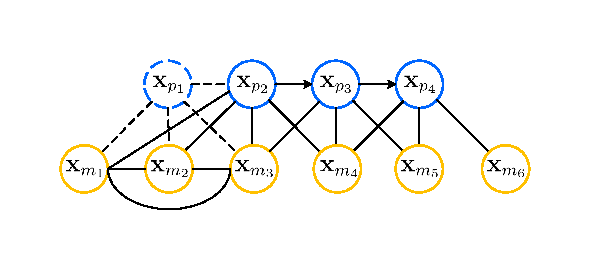
\includegraphics[width=0.15\textwidth, angle=-90]{figures/chapter4/fig4_4}
	\caption{边缘化掉 $\mathbf{x}_{p_1} $ 后位姿和路标点的关系}\label{fig4_4}
\end{figure}

观察图\ref{fig4_4}可以发现,路标点 $\mathbf{x}_{m_1},  \mathbf{x}_{m_2}, \mathbf{x}_{m_3} $ 之间已经相互有了新的联系,并且,位姿 $\mathbf{x}_{p_2} $ 与路标点 $\mathbf{x}_{m_2} $ 也有了新的联系。这些新的联系就是新的约束项,表现在图\ref{fig4_3}(c)中的黄色区域。

图\ref{fig4_3}(d)是表示再次边缘化掉路标点 $\mathbf{x}_{m_1} $ 后的 $\mathbf{H} $ 矩阵,其对应的关系图如图\ref{fig4_5}所示。
\begin{figure}[h]\setlength{\belowcaptionskip}{1pt}
	\centering
	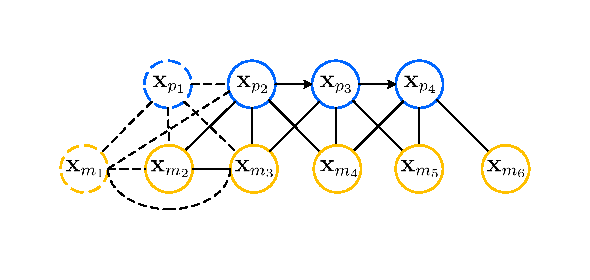
\includegraphics[width=0.15\textwidth, angle=-90]{figures/chapter4/fig4_5}
	\caption{边缘化掉 $\mathbf{x}_{p_1} $ 和$\mathbf{x}_{m_1} $ 后位姿和路标点的关系}\label{fig4_5}
\end{figure} 
\begin{figure}[h]\setlength{\belowcaptionskip}{-12pt}
	\centering
	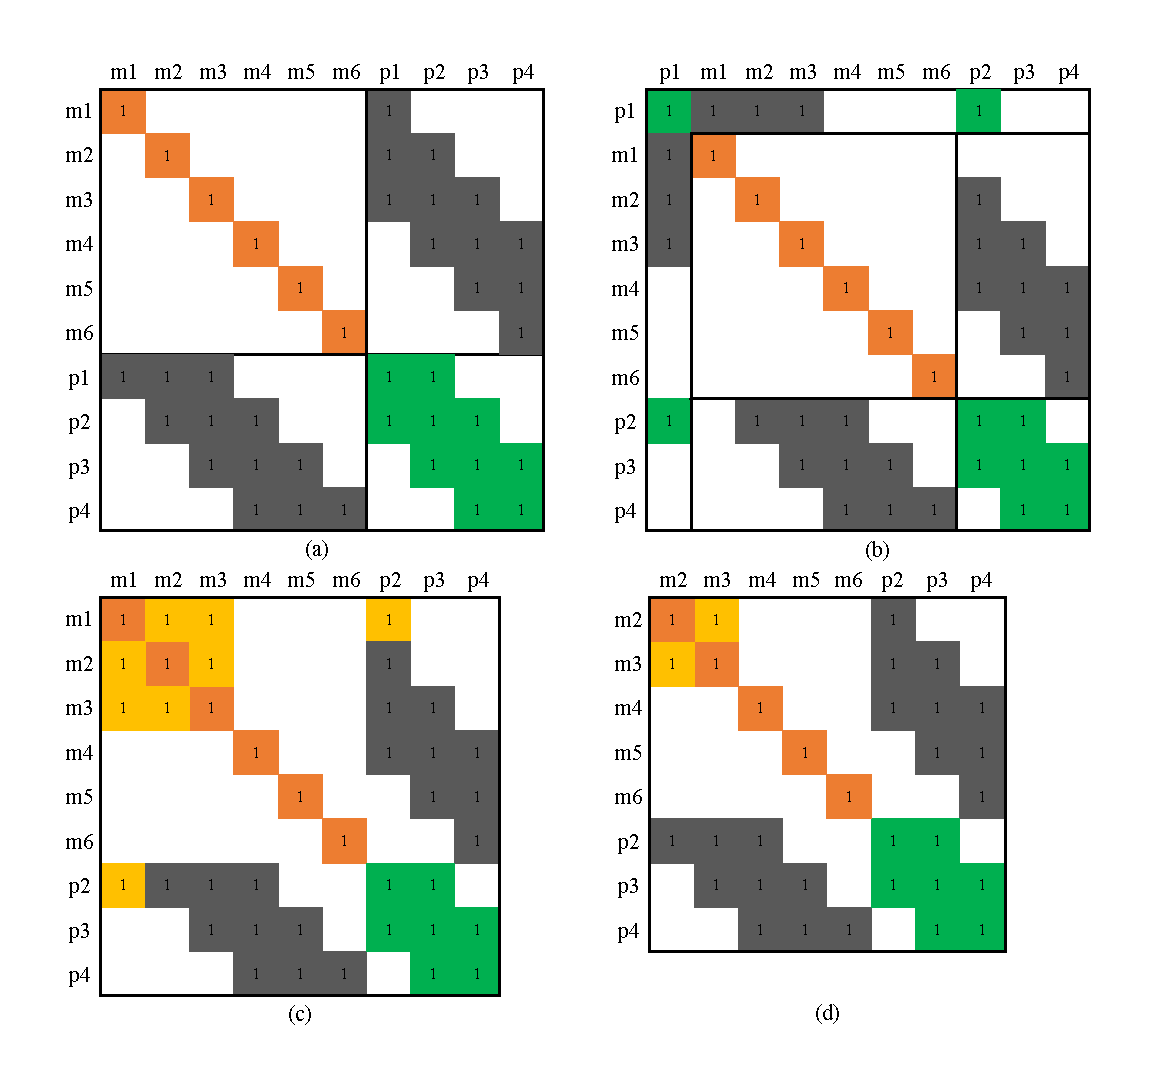
\includegraphics[width=0.75\textwidth, angle=-90]{figures/chapter4/fig4_3}
	\caption{边缘化过程中 $\mathbf{H} $ 矩阵变化图}\label{fig4_3}
\end{figure}
观察图\ref{fig4_3}(d),发现$\mathbf{H} $ 矩阵并没有变得更稠密,这是因为路标点 $\mathbf{x}_{m_1} $ 本身就没有被其他路标点观测到(从图\ref{fig4_4}中可以看出),也就不会与其他位姿产生约束关系。因此,可以得出一个结论:当边缘化掉不被其他帧所观测到的路标点时,$\mathbf{H} $ 矩阵不会进一步稠密。而对于被其他帧所观测到的路标点,通常不进行边缘化。

3. 滑窗策略
\begin{figure}[h]\setlength{\belowcaptionskip}{-12pt}
	\centering
	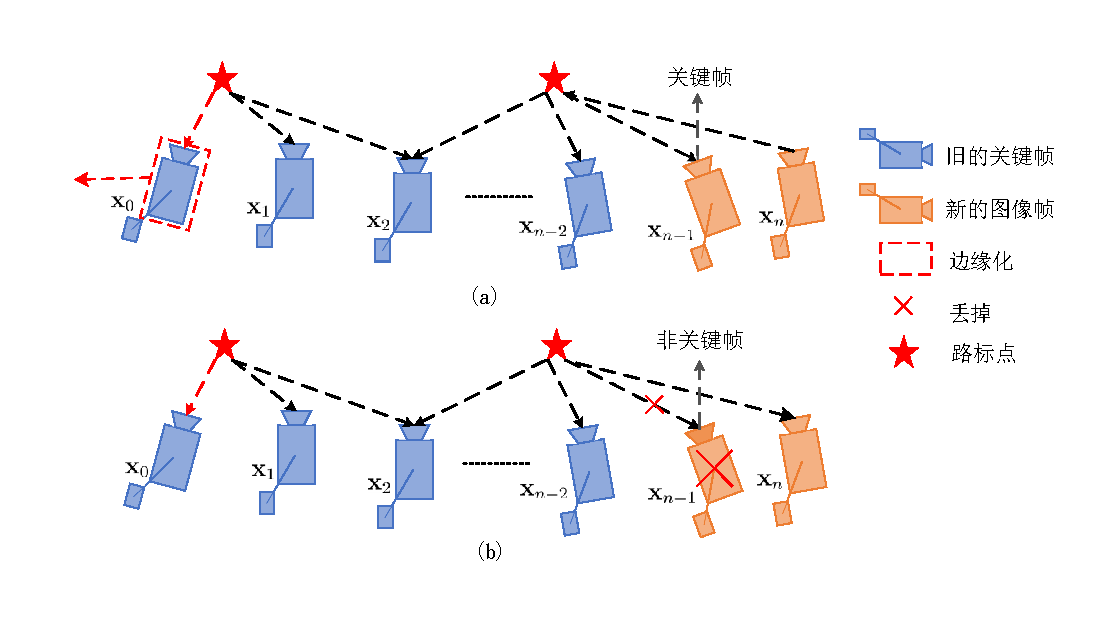
\includegraphics[width=0.4\textwidth, angle=-90]{figures/chapter4/fig4_6}
	\caption{滑动窗口示意图}\label{fig4_6}
\end{figure}

如图\ref{fig4_6}所示,整个后端非线性优化采用滑动窗口机制,窗口内维持固定的图像帧数量,根据新到来的图像帧是否为关键帧,使用不同的处理机制。图中$\mathbf{x}_n $ 为最新的图像帧, $\mathbf{x}_{n-1} $为次新帧图像,$\mathbf{x}_{n-2} $ 为第一帧旧的图像帧, $\mathbf{x}_{0} $为最旧的图像帧。

(1)如果 $\mathbf{x}_{n-1} $ 是关键帧,对 $\mathbf{x}_{0} $进行边缘化处理,与 $\mathbf{x}_{0} $及其关联的路标点的约束信息将转变为先验信息并整合到目标函数中;

(2)如果 $\mathbf{x}_{n-1} $不是关键帧,将 $\mathbf{x}_{n-1} $及其观测到的路标点直接丢弃。如果$\mathbf{x}_{n-1} $ 不是关键帧,说明它跟$\mathbf{x}_{n-2} $ 很相似(通过视差来判断是否为关键帧),那么$\mathbf{x}_{n-1} $ 及其路标点具有的约束信息和$\mathbf{x}_{n-2} $ 几乎一样,所以直接丢掉$\mathbf{x}_{n-1} $ 也不会丢失很多的约束信息。

需要注意的是,不管是边缘化还是直接丢弃图像帧,都会完整的保留图像帧所对应的IMU预积分信息,从而确保IMU预积分不中断。
\section{闭环检测}
上一章研究了前端、初始化和后端优化,此时是视觉和IMU已经构成了紧耦合的VIO系统,能够估计出自身的位姿和路标点的位置。此时的VIO系统虽然可以对自身进行定位,但是由于视觉和IMU都有不可避免的累计误差,所以在融合之后的系统还是有误差的。这就导致了系统长时间估计的结果是不可靠的,无法构建全局一致(Global Consistent)的轨迹和地图。

闭环检测算法可以检测相机是否回到了之前的位置,如果检测到闭环,算法会将之前的累计误差消除掉,将轨迹拉回正确的位置,从而构建全局一致的轨迹和地图。而且,闭环检测能够给出当前图像与之前所有图像之间的关联信息,所以,如果在前端特征跟丢的情况下,可以通过闭环检测对当前的位置进行重定位,从而不至于使系统崩溃。
\subsection{词袋模型}
闭环检测有两种思路:基于里程计的几何关系和基于外观。基于里程计的几何关系是指,当相机运动到以前走过的某个位置附近时,检测是否存在闭环\upcite{hahnel2003efficient}。这种方法有一个致命问题,长时间的视觉里程计的累计误差会导致轨迹严重漂移,相机自身是无法分辨出是否回到之前的某个位置,也就无法判断是否存在闭环关系。因此这种方法仅仅适用于短距离,短时间的闭环运动。

第二种方法是基于外观的。它仅仅依靠图像间的相似程度来确定是否存在闭环关系。这种方法不受前端累计误差的影响,使得闭环检测可以独立的作为系统的一个模块。基于外观的方法是视觉SLAM中检测闭环的主流做法,并且已经应用于多个实际系统中\upcite{ulrich2000appearance}\upcite{latif2013robust}\upcite{mur2015orb}。

如果使用第二种方法,那么闭环检测的关键就在于如何计算图像之间的相似程度。对于任意两张图像 $\bm{A} $ 和 $\bm{B} $ ,会用一种方法计算出他们之间的相似性评分:$s(\bm{A}, \bm{B}) $ 。设定一个阈值,当评分大于这个阈值的时候,就认为他们之间存在闭环关系。通常,采用词袋模型(Bag-of-Words,BoW)\upcite{filliat2007visual}\upcite{galvez2012bags}来计算相似性评分。

词袋是用来描述图像内容特征的方法。图像中出现的一类物体(比如车,房子,人等)会对应于词袋中的一个“单词”,所有的单词构成一个“字典”。通常找出图像中出现了那些“单词”,出现单词的地方用“1”表示,没有出现的用“0”表示,所有的单词出现情况会构成一个向量,然后用这个向量来描述这张图像。最后,用向量的相似程度来表示图像间的相似程度。

假如有一个“字典”,字典里面的单词包括:“汽车”,“行人”和“房子”,分别记为$w_1,w_2,w_3 $ 。有一副图像 $\bm{A} $ 包含了“汽车”和“行人”,没有“房子”,图像$\bm{B} $ 包含了“汽车”和“房子”,没有“行人”那么 $\bm{A},\bm{B} $ 可以表示为:
\begin{equation}
\label{eqn:4.27}
\setlength{\abovedisplayskip}{6pt}
\setlength{\belowdisplayskip}{6pt}
\begin{aligned}
\bm{A}&=1 \cdot w_{1}+1 \cdot w_{2}+0 \cdot w_{3}, \\
\bm{B}&=1 \cdot w_{1}+0 \cdot w_{2}+1 \cdot w_{3}
\end{aligned}
\end{equation}

所以,可以用向量 $[1,1,0]^{T} $ 来表示图像 $\bm{A} $ ,向量$[1,0,1]^{T} $ 来表示图像 $\bm{B} $。可以发现,词袋模型描述的是图像中是否存在某个物体,而不管他们出现在图像的哪个地方。根据这两个向量来计算相似性:
\begin{equation}
\label{eqn:4.28}
\setlength{\abovedisplayskip}{6pt}
\setlength{\belowdisplayskip}{6pt}
s(\boldsymbol{A}, \boldsymbol{B})=1-\frac{1}{W}\|\boldsymbol{A}-\boldsymbol{B}\|_{1}
\end{equation}
其中 $W $是词袋中“单词”的个数,这里 $W =3$,当然,实际中的 $W $会大得多。 $||\cdot || $代表$L_1 $ 范数,也可以选用其他范数,依据具体情况而定。可以发现,当向量 $\bm{A},\bm{B} $ 完全一样时,$s=1$ ;完全相反时,$s=0$ 。这样就可以用 $s$ 的大小来描述图像的相似性了。
\subsection{字典构建}
字典是由“单词”构成,而单词是从图像中抽象而来的。一个“单词”往往是一类特征的集合,所以可以通过聚类(Clustering)来确定“单词”。

聚类属于无监督机器学习(Unsupervised ML),用来寻找大量数据中的规律。假设在前端提取了 $N$个特征,想要从这$N$ 个特征中抽象出来$k$ 个“单词”。使用K均值(K-means)\upcite{jain2010data}算法来解决该问题:

(1)在 $N$ 个特征中随机选取 $k$ 个特征作为中心点:$c_{1}, \dots, c_{k} $ ;

(2)对其他的每个特征,计算它和每个中心点之间的距离,将它与距离最小的那个中心点归为一类;

(3)再次计算每个类的中心点;

(4)如果重新计算出来的中心点和之前的中心点相差不大,则说明算法收敛,聚类成功。否则,返回到步骤(1)。

至此,就可以得到一个字典了。接下来要考虑的是如何根据图像中提取的特征和字典中的“单词”进行匹配。最简单的方法是采取暴力匹配,将特征和字典中的每个“单词”进行匹配,取相似度最高的那个。然而,字典一般是通用性的,这就意味着字典中含有很多的单词,暴力匹配会很耗时。

为了解决这个问题,将字典表示称 $k$ 叉树。$k$ 叉树将聚类层次化,是k均值的一种扩展。如图\ref{fig4_7}所示,用刚才的 $N$ 个特征构建一个深度为 $d$ ,树杈为 $k$ 的树:

(1)用k均值法将根节点(所有的 $N$ 个特征)聚成 $k$ 类,得到第一层聚类;

(2)对第一层聚类的每个节点,再使用k均值法聚成 $k$ 类,得到第二层聚类;

(3)以此类推,直到第 $k-1$ 层聚类,也就是叶子节点,此时的每个叶子节点就是一个“单词”。

可以发现深度为 $d$ ,分支为 $k$ 的树,可以最终聚类成 $k^d$ 个单词。在查找“单词”时,只需要查找每一个中间层聚类的聚类中心,总共需要查找 $d$ 次。
\begin{figure}[h]\setlength{\belowcaptionskip}{-12pt}
	\centering
	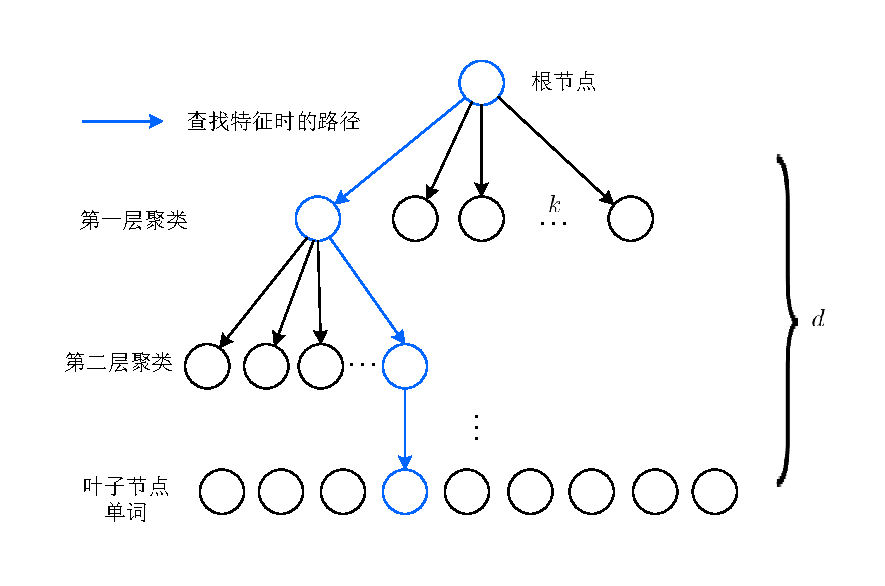
\includegraphics[width=0.4\textwidth, angle=-90]{figures/chapter4/fig4_7}
	\caption{K叉树字典示意图}\label{fig4_7}
\end{figure}
\subsection{相似度计算}
在研究词袋模型的时候简单研究了一种计算相似度的方法,那是一种简单的为了帮助理解的方法。实际中,会用到另一种方法。在之前研究的计算方法中,对所有的“单词”都同等对待,有就是“1”,没有就是“0”。但是,实际中,不同的“单词”在区分性上不相同。比如,在空旷的野外,像“树木”,“花草”,“高山”等类的“单词”会在图像中经常出现,无法根据他们判断该图像跟其他图像的区别。但是如果有“房屋”,“汽车”等类的“单词”出现时,将更容易的判断出该图像相对于其他图像的独特之处。可以说,他们提供了区分度更大的信息。所以,需要对每个单词的区分度有一个量化的评估,通常使用加权的方法来区别不同单词的重要性。权重越大,区分度就越高。

在文本检索领域,TF-IDF(Term Frequency–Inverse Document Frequency)是一种常见的方法\upcite{sivic2003video}\upcite{robertson2004understanding}。TF表示,如果文本中经常出现一个单词,则它的区分度相对较好。IDF表示,文本中出现的相似单词越少,与其他文本的区别就越大。在闭环检测中可以借鉴此方法。

对于词袋模型,在构建词典时,借鉴IDF思想。计算某个“单词” $w_i$ 中的特征数量与所有特征总数的比值,将这个比值作为IDF。设 $w_i$ 的特征数量为 $n_i$ ,特征总数为 $n$ ,那么 $w_i$ 的IDF为:
\begin{equation}
\label{eqn:4.29}
\setlength{\abovedisplayskip}{6pt}
\setlength{\belowdisplayskip}{6pt}
\mathrm{IDF}_{i}=\log \frac{n}{n_{i}}
\end{equation}
另一方面,对于单个图像,借鉴TF思想。设图像 $\bm{A} $ 中,“单词” $w_i$ 出现了 $m_i$ 次,出现的单词总数为 $m$ ,那么 $w_i$ 的TF为:
\begin{equation}
\label{eqn:4.30}
\setlength{\abovedisplayskip}{6pt}
\setlength{\belowdisplayskip}{6pt}
\mathrm{TF}_{i}=\frac{m_{i}}{m}
\end{equation}
定义 $w_i$ 的权重为:
\begin{equation}
\label{eqn:4.31}
\setlength{\abovedisplayskip}{6pt}
\setlength{\belowdisplayskip}{6pt}
\eta_{i}=\mathrm{TF}_{i} \times \operatorname{IDF}_{i}
\end{equation}
有了每个“单词”的权重,可以计算该图像的词袋(用向量 $\bm{v}_A $ 表示):
\begin{equation}
\label{eqn:4.32}
\setlength{\abovedisplayskip}{6pt}
\setlength{\belowdisplayskip}{6pt}
\bm{v}_{A}  \triangleq 
\left\{\left(w_{1}, \eta_{1}\right),\left(w_{2}, \eta_{2}\right), \ldots,\left(w_{N}, \eta_{N}\right)\right\}
\end{equation}
 $\bm{v}_A $是一个稀疏向量,其非零部分(TF-IDF的值)表示图像中包括哪些“单词”。
 
 假设计算出了图像 $\bm{A} $ 和 $\bm{B} $ 的词袋: $\bm{v}_A $和$\bm{v}_B $ ,那么可以定义他们之间的相似度为:
 \begin{equation}
 \label{eqn:4.33}
 s\left(\boldsymbol{v}_{A}-\boldsymbol{v}_{B}\right)=2 \sum_{i=1}^{N}\left|\boldsymbol{v}_{A i}\right|+\left|\boldsymbol{v}_{B i}\right|-\left|\boldsymbol{v}_{A i}-\boldsymbol{v}_{B i}\right|
  \end{equation}
  当然相似度的计算方法有很多种,这里采用 $L_1 $ 范数形式。
  
  在滑动窗口策略中,会实时计算当前帧与字典里词袋的相似度分数,并与之前的所有关键帧进行比较,并对其实施闭环一致性检验,从而得到闭环候选帧。
\subsection{闭环检测方案}
本系统采用基于BRIEF描述子的DboW2词袋进行闭环检测。在视觉前端通常会检测出100 \textasciitilde 150个左右个FAST角点,这对于闭环检测来说是远远不够的。因此会对滑动窗口中滑出的关键帧(即非线性优化处理完的帧)再次提取出500个左右的FAST角点,同时计算所有角点的BRIEF描述子。然后计算当前帧与词袋的相似度分数,并于关键帧数据库中的所有关键帧对比,进行闭环一致性检测,获得闭环候选帧。

检测到闭环后,利用BRIEF描述子对闭环候选帧中旧帧的500个FAST角点和当前帧中的100 \textasciitilde 150个FAST角点进行基于描述子的邻域匹配,如果匹配的点对大于设定的阈值,则利用基础矩阵进行RANSAC异常点剔除。如果经过异常点剔除后的匹配点仍然超过设定的阈值,则认为该候选帧是一个正确的闭环帧。
\section{重定位和闭环优化}
\subsection{重定位}
在后端采用的滑动窗口和边缘化方案极大的降低了计算的复杂性,但也给系统带来了累积误差。更确切地说,累积误差主要发生在全局三维位置 $(x,y,z) $ 和与重力方向垂直的偏航角上。为了减少误差,提出了一种利用闭环检测来矫正误差图像位置的重定位方法。

如图\ref{fig4_8}所示,通过闭环检测建立闭环候选帧(蓝色的帧)和当前滑动窗口中的图像帧(绿色的帧)之间的特征关系。当检测到闭环时,将当前帧的位姿及其对应的路标点作为视觉约束项,并添加到目标函数中。所以式(4.2)可以重新写为:
 \begin{equation}
\label{eqn:4.34}
\begin{split}
\underset{\mathcal{X}}{\text{min}}\left\{\left\| \mathbf{r}_p-\mathbf{H}_p\mathcal{X} \right\|^2+
\sum_{k\in\mathcal{B}}\left\| \mathbf{r}_\mathcal{B}(\hat{\mathbf{z}}_{b_{k+1}}^{b_k},\mathcal{X}) \right\|
_{\mathbf{p}_{b_{k+1}}^{b_k}}^2 \right.  + 
\sum_{(l,j)\in\mathcal{C}}\rho(\left\| \mathbf{r}_\mathcal{C}(\hat{\mathbf{z}}_l^{c_j},\mathcal{X}) 
\right\|_{\mathbf{p}_l^{c_j}}^2) \\ + 
\left.\sum_{(l,j)\in\mathcal{L}}\rho(\left\|\mathbf{r}_\mathcal{C}(\hat{\mathbf{z}}_l^v,\mathcal{X},\hat{\mathbf{q}}_v^w,\hat{\mathbf{p}}_v^w) \right\|_{\mathbf{p}_l^{c_v}}^2) \right\}
\end{split}
\end{equation}
其中 $(\hat{\mathbf{q}}_v^w,\hat{\mathbf{p}}_v^w) $ 是回环帧的姿态,被视为常数。$\mathcal{L} $ 是闭环帧中检索到的路标点的集合。$(l,v) $ 是指在闭环帧 $v $ 中观察到的第 $l $ 个特征。注意,虽然目标函数与之前略有不同,但待解状态量的维数保持不变,因为回环帧的姿态被视为常数。当滑动窗口建立多个回环时,使用来自所有闭环帧及其对应的路标点进行优化。这就为重新定位提供了多视角的约束,从而提高了定位的精度和平滑性。
\begin{figure}[h]\setlength{\belowcaptionskip}{-12pt}
	\centering
	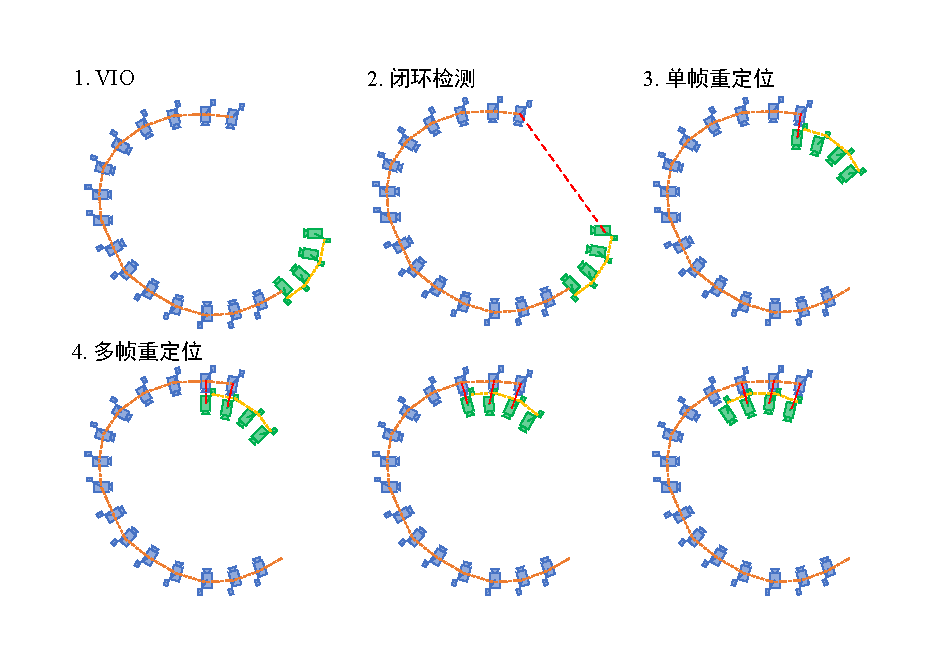
\includegraphics[width=0.4\textwidth, angle=-90]{figures/chapter4/fig4_8}
	\caption{重定位过程示意图}\label{fig4_8}
\end{figure}
\subsection{闭环优化}
之前讨论的BA优化,往往是同时优化位姿及其3D路标点,这样会存在一个问题:随着时间的累计,相机的运动距离越来越远,路标点也在不断增加,如果不使用滑窗优化,而是优化过去所有的位姿和路标点,那么计算量会逐渐增加,计算效率会逐渐下降。当然,本系统中使用了滑窗策略,避免了这种情况。为了达到全局一致性的目的,当检测到闭环的时候,需要进行一次全局优化。为了避免极低的计算效率,采用位姿图优化,而不是全局BA优化。位姿图优化,只对位姿进行优化,而忽略路标点。通常路标点经过多次观测优化后会收敛到一个固定值,而那些发散的异常点会消失不见。对于那些收敛的点,不需一直进行优化。在闭环之前,路标点肯定都经过了多次优化,已经收敛,所以闭环的时候没有必要再次优化,而只需要优化位姿即可。

图优化是由节点和边构成的,节点是待优化的变量,边是约束关系。那么位姿图呢?位姿图的节点表示相机位姿,用李代数 $ \bm{ \xi}_{1}, {\ldots}, \bm{\xi}_{n} $ 表示,位姿图的边是位姿间相机的运动,用 $\Delta \boldsymbol{\xi}_{i j} $ 表示位姿 $\bm{\xi}_{i} $和$\bm{\xi}_{i} $ 之间的相机运动,则,
\begin{equation}
\label{eqn:4.35}
\setlength{\abovedisplayskip}{6pt}
\setlength{\belowdisplayskip}{6pt}
\Delta \boldsymbol{\xi}_{i j}=\boldsymbol{\xi}_{i}^{-1} \circ \boldsymbol{\xi}_{j}=\ln \left(\exp \left(\left[-\boldsymbol{\xi}_{i}\right]_\times \right) \exp \left(\left[\boldsymbol{\xi}_{j}\right]_\times\right)\right)^{\vee}
\end{equation}
或者可以用李群表示为:
\begin{equation}
\label{eqn:4.36}
\setlength{\abovedisplayskip}{6pt}
\setlength{\belowdisplayskip}{6pt}
\Delta \boldsymbol{T}_{i j}=\boldsymbol{T}_{i}^{-1} \boldsymbol{T}_{j}
\end{equation}
上式中的“=”不完全成立,将利用这个误差来构建残差项:
\begin{equation}
\label{eqn:4.37}
\setlength{\abovedisplayskip}{6pt}
\setlength{\belowdisplayskip}{6pt}
\begin{aligned} 
	\boldsymbol{e}_{i j} &=\ln \left(\Delta \boldsymbol{T}_{i j}^{-1} \boldsymbol{T}_{i}^{-1} \boldsymbol{T}_{j}\right)^{\vee} \\ 
	&=\ln \left( \exp \left(\left[-\boldsymbol{\xi}_{i j}\right]_\times \right) \exp \left(\left[-\boldsymbol{\xi}_{i}\right]_\times\right) \exp \left( \left[\boldsymbol{\xi}_{j}\right]_\times \right)\right)^{\vee} 
\end{aligned}
\end{equation}

按照前面研究优化的思路,需要求残差对优化变量的一阶导数,仍旧用扰动求导的方式:
\begin{equation}
\label{eqn:4.38}
\setlength{\abovedisplayskip}{6pt}
\setlength{\belowdisplayskip}{6pt}
\hat{\boldsymbol{e}}_{i j}=
\ln \left(\boldsymbol{T}_{i j}^{-1} \boldsymbol{T}_{i}^{-1} \exp \left(\left[-\boldsymbol{\delta} \boldsymbol{\xi}_{i}\right]_\times\right) 
\exp \left(\left[\delta \boldsymbol{\xi}_{j}\right]_\times\right) \boldsymbol{T}_{j}\right)^{\vee}
\end{equation}
其中 $\delta \bm{\xi}_{i} $和 $\delta \bm{\xi}_{j} $为 $\bm{\xi}_{i}  $和 $\bm{\xi}_{j}  $的左扰动。根据李群上的伴随性质,即
\begin{equation}
\label{eqn:4.39}
\setlength{\abovedisplayskip}{6pt}
\setlength{\belowdisplayskip}{6pt}
\exp \left(\left[\operatorname{Ad}(\boldsymbol{T}) \boldsymbol{\xi}\right]_\times\right)=
\boldsymbol{T} \exp \left( \left[\boldsymbol{\xi}\right]_\times\right) \boldsymbol{T}^{-1}
\end{equation}
其中
\[\operatorname{Ad}(\boldsymbol{T})=\left[ \begin{array}{cc}{\boldsymbol{R}} & {\left[\boldsymbol{t}\right]_\times \boldsymbol{R}} \\ {0} & {\boldsymbol{R}}\end{array}\right]\]
可得:
\begin{equation}
\label{eqn:4.40}
\exp \left( \left[\boldsymbol{\xi}\right]_\times\right) \boldsymbol{T}=
\boldsymbol{T} \exp \left(\left[\operatorname{Ad}\left(\boldsymbol{T}^{-1}\right) \boldsymbol{\xi}\right]_\times\right)
\end{equation}
利用式(\ref{eqn:4.40}),将扰动移到最右侧,从而推导出右乘雅可比矩阵:
\begin{equation}
\label{eqn:4.41}
\begin{aligned} 
\hat{\bm{e}}_{i j} &=
\ln \left\{
\boldsymbol{T}_{i j}^{-1} \boldsymbol{T}_{i}^{-1} 
\exp \left( \left[-\delta \boldsymbol{\xi}_{i}\right]_\times \right) 
\exp \left( \left[\delta \boldsymbol{\xi}_{j}\right]_\times \right) \boldsymbol{T}_{j}
\right\}^{\vee} \\
&=
\ln \left\{
\boldsymbol{T}_{i j}^{-1} \boldsymbol{T}_{i}^{-1} \boldsymbol{T}_{j} 
\exp \left(
\left[-\mathrm{Ad}\left(\boldsymbol{T}_{j}^{-1}\right) \boldsymbol{\delta} \boldsymbol{\xi}_{i}\right]_\times
\right) 
\exp \left(
\left[\mathrm{A} \mathrm{d}\left(\boldsymbol{T}_{j}^{-1}\right) \boldsymbol{\delta} \boldsymbol{\xi}_{j}\right]_\times
\right)
\right\} ^ {\vee}\\
& \approx \boldsymbol{e}_{i j} + \frac{\partial \boldsymbol{e}_{i j}}{\partial \delta \xi_{i}} \boldsymbol{\delta} \boldsymbol{\xi}_{i} 
+ \frac{\partial \boldsymbol{e}_{i j}}{\partial \delta \xi_{j}} \boldsymbol{\delta} \boldsymbol{\xi}_{j}
\end{aligned}
\end{equation}
其中
\begin{equation}
\label{eqn:4.42}
\begin{aligned}
\frac{\partial \boldsymbol{e}_{i j}}{\partial \delta \xi_{i}} &= -\bm{\mathcal{J}}_{r}^{-1}\left(\boldsymbol{e}_{i j}\right) \operatorname{Ad}\left(\boldsymbol{T}_{j}^{-1}\right) \\
\frac{\partial \boldsymbol{e}_{i j}}{\partial \boldsymbol{\delta} \xi_{j}} &= \bm{\mathcal{J}}_{r}^{-1}\left(\boldsymbol{e}_{i j}\right) \operatorname{Ad}\left(\boldsymbol{T}_{j}^{-1}\right)
\end{aligned}
\end{equation}
一般李代数上的雅可比矩阵比较复杂,通常近似取为:
\begin{equation}
\label{eqn:4.43}
\bm{\mathcal{J}}_{r}^{-1}\left(\boldsymbol{e}_{i j}\right) \approx 
\boldsymbol{I}+\frac{1}{2} \left[ 
\begin{array}{cc}
{\left[\boldsymbol{\phi}_{\boldsymbol{e}} \right]_\times} & { \left[ \boldsymbol{\rho}_{\boldsymbol{e}} \right]_\times } \\ 
{\mathbf{0}} & { \left[\bm{\phi}_{\boldsymbol{e}}\right]_\times}
\end{array}
\right]
\end{equation}
到此为止,求的仅仅是位姿图中的一条边的残差,记所有边的集合为 ,那么所有边的残差就构成了目标函数:
\begin{equation}
\label{eqn:4.44}
\min _{\bm{\xi}} \frac{1}{2} \sum_{i, j \in \mathcal{E}} \bm{e}_{i j}^{T} \Sigma_{i j}^{-1} \bm{e}_{i j}
\end{equation}
然后用高斯-牛顿或者LM方法迭代求解最优值。

在本系统中,当检测到闭环的时候,进行全局位姿优化。这里的位姿指3自由度位置 $(x,y,z) $和一个偏航角 $\hat{\psi}_{ij} $,总共四自由度。忽略横滚角和俯仰角是因为在单目/视觉惯性融合系统中,这两个角度是可以根据重力的方向观测到的,不会产生累计漂移。

当滑动窗口中最旧的那一帧关键帧滑出窗口时,它将被添加到位姿图中。该关键帧是位姿图的顶点,它通过两条边和其他顶点相连:

(1)第一条边是滑动窗口中的两个关键帧之间的相对变换(或者叫相对位姿),称为序列边。假设关键帧 $i$ 是最新进行边缘化的帧,其之前的某一个关键帧为 $j$ ,那么序列边为包括 $i$ 和 $j$ 的相对位移 $\hat{\mathbf{p}}_{ij}^i $ 以及偏航角 $\hat{\psi}_{ij} $ :
\begin{equation}
\label{eqn:4.45}
\setlength{\abovedisplayskip}{6pt}
\setlength{\belowdisplayskip}{6pt}
\begin{split}
\hat{\mathbf{p}}_{ij}^i&=\hat{\mathbf{R}}_i^{w^{-1}}(\hat{\mathbf{p}}_j^w-\hat{\mathbf{p}}_i^w) \\
\hat{\psi}_{ij}&=\hat{\psi}_j-\hat{\psi}_i.
\end{split}
\end{equation}

(2)第二条边是检测到闭环后形成的闭环边。其定义和式(\ref{eqn:4.45})一样,通过重定位获得闭环边的值。

有了顶点和边,就可以得到图优化的残差项及目标函数。定义关键帧 $i$ 和 $j$ 之间的残差为:
\begin{equation}
\label{eqn:4.46}
\mathbf{r}_{i,j}(\mathbf{p}_i^w,\psi_i,\mathbf{p}_j^w,\psi_j)=\begin{bmatrix}
\mathbf{R}(\hat{\phi}_i,\hat{\theta}_i,\psi_i)^{-1}(\mathbf{p}_j^w-\mathbf{P}_i^w)-\hat{\mathbf{p}}_{ij}^i \\
\psi_j-\psi_i-\hat{\psi}_{ij}
\end{bmatrix}
\end{equation}
其中$\hat{\phi}_i,\hat{\theta}_i $ 是单目VIO估计出的横滚角和俯仰角。

所有的序列边和闭环边的残差项之和构成了整体的目标函数:
\begin{equation}
\label{eqn:4.47}
\begin{split}
\underset{\mathcal{\mathbf{p},\psi}}{\text{min}}
\left\{
\sum_{(i,j)\in\mathcal{S}}\left\| \mathbf{r}_{i,j} \right\|^2+\sum_{(i,j)\in\mathcal{L}}\rho(\left\| \mathbf{r}_{i,j} \right\|^2)
\right\}
\end{split}
\end{equation}
其中 $\mathcal{S} $ 是所有序列边的集合,$\mathcal{L} $ 是所有闭环边的集合。$\rho(\cdot) $  是Huber范数。对闭环边使用Huber范数是为了减少错误闭环的影响,而对于序列边不使用Huber范数,因为序列边是VIO给出的,VIO已经经行了“异常点”剔除。

位姿图优化和重新定位将异步运行在两个独立的线程中,以便在进行重定位时,能立即使用最优化的位姿图。同样,即使当前的姿态图优化尚未完成,仍然可以使用现有的姿态图进行重定位。这一过程如图\ref{fig4_9}所示。
\begin{figure}[h]\setlength{\belowcaptionskip}{-12pt}
	\centering
	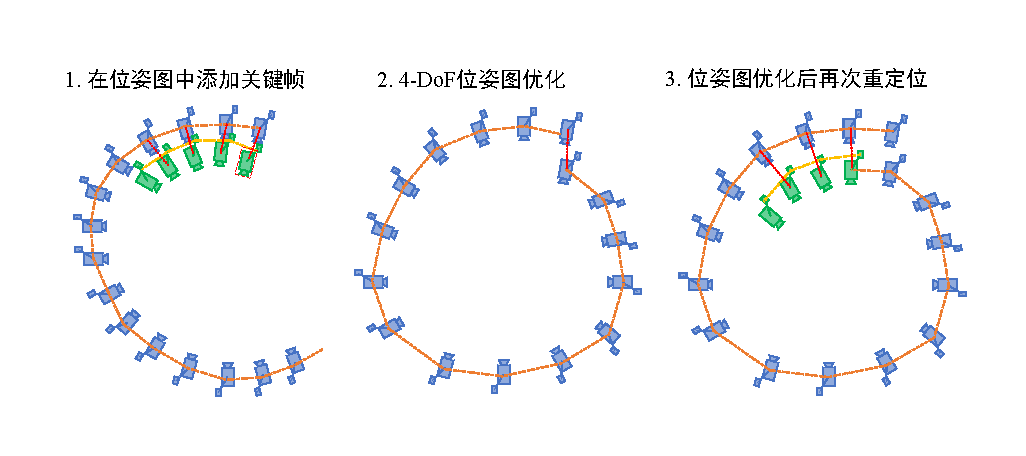
\includegraphics[width=0.3\textwidth, angle=-90]{figures/chapter4/fig4_9}
	\caption{位姿优化示意图}\label{fig4_9}
\end{figure}
\section{本章小结}
本章对系统的后端优化和闭环检测算法进行了详细的阐述。首先研究了后端优化的优化变量、目标函数以及构成目标函数的各个残差项,并解释了边缘化过程。然后研究了基于词袋模型的闭环检测算法。最后分析了重定位的实现过程,以及基于图优化的闭环优化算法。本章研究的优化算法体现了视觉和IMU之间的紧耦合过程,二者的状态量放在一起进行优化,紧密结合,相辅相成。